\documentclass[11pt]{report}

\usepackage{"../../info/packages"}
\usepackage{"../../info/nomenclature"}
\usepackage{fullpage}


\title{Arbitrary-Lagrangian-Eulerian Finite-Element Hydrodynamics}
\author{Alejandro Campos}

\begin{document}

\maketitle
\tableofcontents

%########################################################################
\chapter{The Lagrangian Step}
%########################################################################
%------------------------------------------------------------------------
\section{Lagrangian governing equations}
%------------------------------------------------------------------------
We consider Lagrangian fluid particles, for which we define their position $\xvec^+=\xvec^+(t,\yvec)$, density $\rho^+ = \rho^+(t,\yvec)$, velocity $\uvec^+ = \uvec^+(t,\yvec)$, and internal energy $e^+ = e^+(t,\yvec)$. The vector $\yvec$ is the location of each fluid particle at time zero and thus serves to differentiate between the different particles. The Eulerian counterparts for the density, velocity, and internal energy are, respectively, $\rho = \rho(t,\xvec)$, $\uvec = \uvec(t,\xvec)$, and $e = e(t,\xvec)$. The vector $\xvec$ is a location in Eulerian space. Also consider the volume $\Omega_0$ as the set of all $\yvec$ vectors that make up the initial domain. The control volume $\Omega^+ = \Omega^+(t, \Omega_0)$ is then defined by
\begin{equation}
    \Omega^+ = \{ \xvec^+:\yvec \in \Omega_0 \}.
\end{equation}
Note that $\Omega^+(0,\Omega_0) = \Omega_0$.

The governing equations for the Lagrangian fluid particles are derived in my fluid-mechanics notes (see section on kinematics, Lagrangian governing equations, etc.). These are shown below
\begin{align}
    \frac{\partial \xvec^+}{\partial t} &= \uvec^+, \label{eq:lag_gov_evol_x} \\
    \frac{\partial \rho^+}{\partial t} &= -\rho^+ \left( \nabla \cdot \uvec \right)_{\xvec = \xvec^+}, \label{eq:lag_gov_evol_rho} \\
    \rho^+ \frac{\partial \uvec^+}{\partial t} &= \left ( \nabla \cdot \sigmavec \right )_{\xvec = \xvec^+}, \label{eq:lag_gov_evol_u} \\
    \rho^+ \frac{\partial e^+}{\partial t} &= \left ( \sigmavec : \nabla \uvec \right )_{\xvec = \xvec^+}. \label{eq:lag_gov_evol_e}
\end{align}
In the above, $\sigmavec = \sigmavec(t,\xvec)$ is the stress tensor.

A note on notation. The products that involve a tensor $\tauvec$ can be expressed in Einstein notation as
\begin{equation*}
    \nabla \cdot \tauvec = \frac{\partial \tau_{ij}}{\partial x_j},
\end{equation*}
\begin{equation*}
    \tauvec \cdot \nabla f = \tau_{ij} \frac{\partial f}{\partial x_j},
\end{equation*}
\begin{equation*}
    \gvec \cdot \tauvec \cdot \nabla f = g_i \tau_{ij} \frac{\partial f}{\partial x_j},
\end{equation*}
\begin{equation*}
    \tauvec : \nabla \gvec = \tau_{ij} \frac{\partial g_i}{\partial x_j}.
\end{equation*}
where $f$ is a scalar and $\gvec$ a vector. In these notes we'll mostly be using indices $i$ and $j$ for FE expansions, rather than for Einstein notation.

%---------------------------------------------------------------
\section{Lagrangian finite elements}
%---------------------------------------------------------------
\label{sec:lag_fin_elem}
We introduce a Lagrangian basis function $\Phi_i^+ = \Phi_i^+(t,\yvec)$ and an Eulerian basis function $\Phi_i = \Phi_i(t,\xvec)$. These are related to each other as any other Lagrangian-Eulerian pair, namely 
\begin{equation}
    \label{eq:lag_fe_phi_correspondence}
    \Phi_i^+(t,\yvec) = \Phi_i(t,\xvec^+(t,\yvec)).
\end{equation}
We now introduce the Lagrangian variable $f^+ = f^+(t,\yvec)$ and the Eulerian counterpart $f = f(t,\xvec)$, and they also satisfy
\begin{equation}
    \label{eq:lag_fe_u_correspondence}
    f^+(t,\yvec) = f(t,\xvec^+(t,\yvec)).
\end{equation}
The expansion of an Eulerian variable in terms of basis functions is as follows
\begin{equation}
    \label{eq:lag_fe_expansion_eul}
    f = \sum_i^n F_i \Phi_i,
\end{equation}
where $F_i = F_i(t)$. Plugging in $\xvec^+$ for $\xvec$ in the above, and using \cref{eq:lag_fe_phi_correspondence,eq:lag_fe_u_correspondence} gives
\begin{equation}
    \label{eq:fe_lag_expansion_lag}
    f^+ = \sum_i^n F_i \Phi_i^+.
\end{equation}
Thus, both the Lagrangian and Eulerian variables share the same finite-element coefficients $F_i$. 

As shown in my fluid mechanics notes, we also have
\begin{equation}
    \label{eq:lag_fe_deriv_correspondence}
    \frac{\partial \Phi_i^+}{\partial t} = \left ( \frac{\partial \Phi_i}{\partial t} + \uvec \cdot \nabla \Phi_i \right )_{\xvec = \xvec^+},
\end{equation}
where $\uvec = \uvec(t,\xvec)$ is the Eulerian counterpart to $\uvec^+$. We'll introduce the restriction that $\Phi_i^+$ is constant in time, that is $\partial \Phi_i^+/\partial t = 0$, which gives
\begin{equation}
    \frac{\partial \Phi_i}{\partial t} + \uvec \cdot \nabla \Phi_i = 0.
\end{equation}
Thus, $F_i$ in \cref{eq:fe_lag_expansion_lag} accounts for the time dependence of $F^+$, whereas $\Phi_i^+$ accounts for the dependence on $\yvec$.

%------------------------------------------------------------------------
\section{Finite element expansion}
%------------------------------------------------------------------------
We introduce the coefficients $\hat{\xvec}_i = \hat{\xvec}_i(t)$, $\hat{\uvec}_i = \hat{\uvec}_i(t)$ and $\hat{e}_i = \hat{e}_i(t)$, as well as the Lagrangian basis functions $\phi^+_i = \phi^+_i(\yvec) \in L^2$, and $w^+_i = w^+_i(\yvec) \in H^1$. We note that $\hat{\xvec}_i$ and $\hat{\uvec}_i$ are each vectors, e.g., the components of $\hat{\uvec}_i$ are $\hat{u}_{i,\alpha} = \hat{u}_{i,\alpha}(t)$ for $\alpha = x,y,z$. We also note that $\phi^+_i$ and $w^+_i$ have Eulerian counterparts $\phi_i = \phi_i(t,\xvec)$ and $w_i = w_i(t,\xvec)$, respectively. The coefficients are used in the following expansions
\begin{equation}
    \label{eq:fe_exp_x}
    \xvec^+ = \sum_j^{N_w} \hat{\xvec}_j w^+_j,
\end{equation}
\begin{equation}
    \label{eq:fe_exp_u}
    \uvec^+ = \sum_j^{N_w} \hat{\uvec}_j w^+_j,
\end{equation}
\begin{equation}
    \label{eq:fe_exp_e}
    e^+ = \sum_j^{N_\phi} \hat{e}_j \phi^+_j.
\end{equation}
We note that the expansion coefficients are the same for the Lagrangian and Eulerian variables, as shown in \cref{sec:lag_fin_elem}. For example, for the Eulerian velocity, we have
\begin{equation}
    \uvec = \sum_j^{N_w} \hat{\uvec}_j w_j.
\end{equation}

%------------------------------------------------------------------------
\section{Semi-discrete Lagrangian governing equations}
%------------------------------------------------------------------------
%---------------------------------
\subsection{Position and Jacobian}
%---------------------------------
Plugging in \cref{eq:fe_exp_x,eq:fe_exp_u} in \cref{eq:lag_gov_evol_x} gives
\begin{equation*}
    \sum_{j}^{N_w} \frac{d \hat{\xvec}_j}{dt} w^+_j = \sum_{j}^{N_w} \hat{\uvec}_j w^+_j.
\end{equation*}
To satisfy the equation above, we'll require
\begin{equation*}
    \frac{d \hat{\xvec}^+_j}{dt} = \hat{\uvec}_j.
\end{equation*}
We now introduce the vectors $\Xvec$ and $\Uvec$, whose components are $\hat{\xvec}_i$ and $\hat{\uvec}_i$, respectively. Thus, the above is written as
\begin{equation}
    \label{eq:evol_x_semi_discrete}
    \frac{d\Xvec}{dt} = \Uvec.
\end{equation}

%---------------------------------
\subsection{Density}
%---------------------------------
We introduce the Jacobian matrix $\Jvec^+ = \Jvec^+(t,\yvec)$, which is defined as 
\begin{equation}
    \Jvec^+ =  \frac{\partial \xvec^+ }{ \partial \yvec}.
\end{equation}
It's determinant is denoted by $J^+ = J^+(t,\yvec)$, and it satisfies the following equation
\begin{equation}
    \label{eq:evol_det_jacob}
    \frac{\partial J^+}{\partial t} = J^+ \left( \nabla \cdot \uvec \right)_{\xvec = \xvec^+}.
\end{equation}
Thus, \Cref{eq:lag_gov_evol_rho} can be re-written as
\begin{equation*}
    \frac{1}{\rho^+} \frac{\partial \rho^+}{\partial t} = -\frac{1}{J^+} \frac{\partial J^+}{\partial t},
\end{equation*}
or
\begin{equation}
    \label{eq:lag_gov_evol_rho_2}
    \frac{\partial J^+ \rho^+}{\partial t} = 0.
\end{equation}
Since $J^+ = 1$ at the initial time, we obtain the density according to
\begin{equation}
    \label{eq:evol_rho_semi_discrete}
    \rho^+ = \frac{\rho^+_0}{J^+},
\end{equation}
where $\rho^+_0 = \rho^+(0,\yvec)$.

To compute $J^+$, we first plug in \cref{eq:fe_exp_x} in the definition of the Jacobian matrix, which gives
\begin{equation*}
    \Jvec^+ = \frac{\partial}{\partial \yvec} \sum_j^{N_w} \hat{\xvec}_j w^+_j = \sum_j^{N_w} \hat{\xvec}_j \nabla_{\yvec} w^+_j.
\end{equation*}
We then simply compute the determinant of the above to obtain $J^+$. Note that for any function $\xvec^+$ and its corresponding $\uvec^+$, whether it be an exact analytical expression or a finite-element expansion as given by \cref{eq:fe_exp_x}, one obtains \cref{eq:evol_det_jacob}. Thus, the derivation of \cref{eq:lag_gov_evol_rho_2} from \cref{eq:lag_gov_evol_rho} still holds whether one plans to represent $J^+$ using an analytical expression or a finite-element expansion. 

%---------------------------------
\subsection{Velocity}
%---------------------------------
Plugging in \cref{eq:evol_rho_semi_discrete} in \cref{eq:lag_gov_evol_u} we get
\begin{equation*}
    \rho^+_0 \frac{\partial \uvec^+}{\partial t} = \left ( \nabla \cdot \sigmavec \right )_{\xvec = \xvec^+} J^+.
\end{equation*}
We then multiply both sides of the above by the basis functions for velocity and integrate over all space to obtain
\begin{equation*}
    \int_{\Omega_0} \rho^+_0 \frac{\partial \uvec^+}{\partial t} w^+_i \, dV_y = \int_{\Omega_0} \left ( \nabla \cdot \sigmavec \right )_{\xvec = \xvec^+} w^+_i J^+ \, dV_y.
\end{equation*}
For the left-hand side we have
\begin{align*}
    \int_{\Omega_0} \rho^+_0 \frac{\partial \uvec^+}{\partial t} w^+_i \, dV_y &= \int_{\Omega_0} \rho^+_0 \sum_j^{N_w} \frac{d \hat{\uvec}_j}{dt} w^+_j w^+_i \, dV_y, \nonumber \\
    &= \sum_j^{N_w} \frac{d \hat{\uvec}_j}{dt} \int_{\Omega_0} \rho^+_0 w^+_i w^+_j \, dV_y, \nonumber \\
    &= \sum_j^{N_w} \frac{d \hat{\uvec}_j}{dt} m_{\mathcal{V},ij},
\end{align*}
where
\begin{equation}
    m_{\mathcal{V},ij} = \int_{\Omega_0} \rho^+_0 w^+_i w^+_j \, dV_y
\end{equation}
is a mass bilinear form (which is independent of time). For the right-hand side we have
\begin{align*}
    \int_{\Omega_0} \left ( \nabla \cdot \sigmavec \right )_{\xvec = \xvec^+} w^+_i J^+ \, dV_y & = \int_{\Omega_0} \left ( \nabla \cdot \sigmavec w_i \right )_{\xvec = \xvec^+} J^+ \, dV_y \nonumber \\
    & = \int_{\Omega^+} \nabla \cdot \sigmavec w_i \, dV_x \nonumber \\
    & = -\int_{\Omega^+} \sigmavec \cdot \nabla w_i \, dV_x.
\end{align*}
The second equality above follows from integration by substitution. Combining results we have
\begin{equation}
    \label{eq:evol_u_semi_discrete}
    \sum_j^{N_w} \frac{d \hat{\uvec}_j}{d t} m_{\mathcal{V},ij} = -\int_{\Omega^+} \sigmavec \cdot \nabla w_i \, dV_x.
\end{equation}

We introduce the matrix $\Mvec_\mathcal{V}$, whose components are $m_{\mathcal{V},ij}$. Thus, the left-hand side of \cref{eq:evol_u_semi_discrete} can be written as $\Mvec_\mathcal{V} \, d\Uvec / dt$.
We also introduce the vector bilinear form
\begin{equation}
    \fvec_{ij} = \int_{\Omega^+} \sigmavec \cdot \nabla w_i \phi_j \, dV_x.
\end{equation}
This is a \textit{vector} bilinear form since $\fvec_{ij}$ has components $f_{ij,\alpha} = f_{ij,\alpha}(t)$, for $\alpha = x,y,z$, where $\alpha$ denotes the first index of $\sigmavec$. We introduce the force matrix $\Fvec$, whose components are $\fvec_{ij}$. We also expand the field with constant value of one as follows
\begin{equation*}
    1 = \sum_i^{N_\phi} \hat{1}_i \phi_i.
\end{equation*}
If we define the vector $\hat{\mathbf{1}}$ as that with components $\hat{1}_i$, we can show that 
\begin{align*}
    \Fvec \hat{\mathbf{1}} &= \sum_j^{N_\phi} \fvec_{ij} \hat{1}_j \nonumber \\
    &= \sum_j^{N_\phi} \int_{\Omega^+} \sigmavec \cdot \nabla w_i \phi_j \, dV_x \hat{1}_j \nonumber \\
    &= \int_{\Omega^+} \sigmavec \cdot \nabla w_i \left ( \sum_j^{N_\phi} \hat{1}_j \phi_j \right ) \, dV_x \nonumber \\
    &= \int_{\Omega^+} \sigmavec \cdot \nabla w_i \, dV_x.
\end{align*}
The above is the negative of the right-hand side of \cref{eq:evol_u_semi_discrete}. Thus, combining all together we get
\begin{equation}
    \label{eq:evol_vel_semi_discrete}
    \Mvec_\mathcal{V} \frac{d\Uvec}{dt} = -\Fvec \hat{\mathbf{1}}.
\end{equation}
We note that since both the Lagrangian and Eulerian velocities share the same coefficients $\Uvec$, we now have a solution for both.

%---------------------------------
\subsection{Energy}
%---------------------------------
Plugging in \cref{eq:evol_rho_semi_discrete} in \cref{eq:lag_gov_evol_e} we get
\begin{equation*}
    \rho^+_0 \frac{\partial e^+}{\partial t} = \left ( \sigmavec : \nabla \uvec \right )_{\xvec = \xvec^+} J^+.
\end{equation*}
We then multiply both sides of the above by the basis functions for energy and integrate over all space to obtain
\begin{equation*}
    \int_{\Omega_0} \rho^+_0 \frac{\partial e^+}{\partial t} \phi_i^+ \, dV_y = \int_{\Omega_0} \left ( \sigmavec : \nabla \uvec \right )_{\xvec = \xvec^+} \phi_i^+ J^+ \, dV_y.
\end{equation*}
For the left-hand side we have
\begin{align*}
    \int_{\Omega_0} \rho^+_0 \frac{\partial e^+}{\partial t} \phi_i^+ \, dV_y &= \int_{\Omega_0} \rho^+_0 \sum_j^{N_\phi} \frac{d \hat{e}_j}{dt} \phi_j^+ \phi_i^+ \, dV_y , \nonumber \\
    &= \sum_j^{N_\phi} \frac{d \hat{e}_j}{dt} \int_{\Omega_0} \rho^+_0 \phi_j^+ \phi_i^+ \, dV_y , \nonumber \\
    &= \sum_j^{N_\phi} \frac{d \hat{e}_j}{dt} m_{\mathcal{E},ij}
\end{align*}
where
\begin{equation}
    m_{\mathcal{E},ij} = \int_{\Omega_0} \rho^+_0 \phi_j^+ \phi_i^+ \, dV_y
\end{equation}
is a mass bilinear form (which is independent of time). For the right-hand side we have
\begin{align*}
    \int_{\Omega_0} \left ( \sigmavec : \nabla \uvec \right )_{\xvec = \xvec^+} \phi_i^+ J^+ \, dV_y &= \int_{\Omega_0} \left ( \sigmavec : \nabla \uvec \phi_i \right )_{\xvec = \xvec^+} J^+ \, dV_y \nonumber \\
    &= \int_{\Omega^+} \sigmavec : \nabla \uvec \phi_i \, dV_x. 
\end{align*}
Combining results we have
\begin{equation*}
    \sum_j^{N_\phi} \frac{d \hat{e}_j}{dt} m_{\mathcal{E},ij} = \int_{\Omega^+} \sigmavec : \nabla \uvec \phi_i \, dV_x.
\end{equation*}
We no show that
\begin{equation*}
    \sigmavec : \nabla \uvec = \sigmavec : \nabla \left ( \sum_k^{N_w} \hat{\uvec}_k w_k \right ) = \sum_k^{N_w} \hat{\uvec}_k \cdot \sigmavec \cdot \nabla w_k,
\end{equation*}
and hence the previous result is written as
\begin{equation*}
    \sum_j^{N_\phi} \frac{d \hat{e}_j}{dt} m_{\mathcal{E},ij} = \sum_k^{N_w} \hat{\uvec}_k \cdot \int_{\Omega^+} \sigmavec \cdot \nabla w_k \phi_i \, dV_x.
\end{equation*}
The above is finally re-written as
\begin{equation}
    \label{eq:evol_e_semi_discrete}
    \sum_j^{N_\phi} \frac{d \hat{e}_j}{d t} m_{\mathcal{E},ij} = \sum_k^{N_w} \hat{\uvec}_k \cdot \fvec_{ki}.
\end{equation}
Note that in the above there is a dot product in the right-hand side, that is, the right-hand side expanded out is  
\begin{equation*}
    \sum_k^{N_w} \hat{\uvec}_k \cdot \fvec_{ki} = \sum_k^{N_w} \sum_{\alpha=x,y,z} \hat{u}_{k,\alpha} f_{ki,\alpha}.
\end{equation*}

We now introduce the vector $\Evec$ whose components are $\hat{e}_i$. We also introduce the matrix $\Mvec_\mathcal{E}$ whose components are $m_{\mathcal{E},ij}$. Thus, \cref{eq:evol_e_semi_discrete} can be succinctly written as
\begin{equation}
    \label{eq:evol_energy_semi_discrete}
    \Mvec_\mathcal{E} \frac{d\Evec}{dt} = \Fvec^T \cdot \Uvec.
\end{equation}
Note again that on the right-hand side above there is a matrix-vector product \textit{and} a dot product. We also note that since both the Lagrangian and Eulerian internal energies share the same coefficients $\Evec$, we now have a solution for both.

%------------------------------------------------------------------------
\section{Momentum and energy conservation}
%------------------------------------------------------------------------
We'll now define the internal energy $IE=IE(t)$, the kinetic energy $KE=KE(t)$, and the momentum $P_\nvec=P_\nvec(t)$ along a constant $\nvec$ direction.
\begin{align}
    IE &= \int_{\Omega^+} \rho e \, dV_x \nonumber \\
    &= \int_{\Omega_0} \rho^+ e^+ J^+ \, dV_y \nonumber \\
    &= \int_{\Omega_0} \rho^+_0 e^+ \, dV_y \nonumber \\
    &= \int_{\Omega_0} \rho_0^+ \sum_{j}^{N_\phi} \hat{e}_j \phi_j^+ \, dV_y \nonumber \\
    &= \int_{\Omega_0} \rho_0^+ \sum_{j}^{N_\phi} \hat{e}_j \phi_j^+ \left ( \sum_{i}^{N_\phi} \hat{1}_i \phi^+_i \right ) \, dV_y \nonumber \\
    &= \sum_i^{N_\phi} \sum_j^{N_\phi} \hat{1}_i \int_{\Omega_0} \rho_0^+ \phi_i^+ \phi_j^+ \, dV_y \hat{e}_j \nonumber \\
    &= \sum_i^{N_\phi} \sum_j^{N_\phi} \hat{1}_i m_{\mathcal{E},ij} \hat{e}_j \nonumber \\
    &= \hat{\mathbf{1}}^T \Mvec_\mathcal{E} \Evec 
\end{align}

\begin{align}
    KE &= \int_{\Omega^+} \frac{1}{2} \rho \uvec \cdot \uvec \, dV_x \nonumber \\
    &= \int_{\Omega_0} \frac{1}{2} \rho^+ \uvec^+ \cdot \uvec^+ J^+ \, dV_y \nonumber \\
    &= \int_{\Omega_0} \frac{1}{2} \rho_0^+ \uvec^+ \cdot \uvec^+ \, dV_y \nonumber \\
    &= \int_{\Omega_0} \frac{1}{2} \rho_0^+ \left ( \sum_i^{N_w} \hat{\uvec}_i w_i^+ \right ) \cdot \left ( \sum_j^{N_w} \hat{\uvec}_j w_j^+ \right ) \, dV_y \nonumber \\
    &= \sum_i^{N_w} \sum_j^{N_w} \frac{1}{2} \hat{\uvec}_i \cdot \int_{\Omega_0}\rho_0^+ w_i^+ w_j^+ \, dV_y \hat{\uvec}_j \nonumber \\
    &= \sum_i^{N_w} \sum_j^{N_w} \frac{1}{2} \hat{\uvec}_i \cdot m_{\mathcal{V},ij} \hat{\uvec}_j \nonumber \\
    &= \frac{1}{2} \Uvec^T \cdot \Mvec_\mathcal{V} \Uvec.
\end{align}

\begin{align}
    P_\nvec &= \int_{\Omega^+} \rho \uvec \cdot \nvec \, dV_x \nonumber \\
    &= \int_{\Omega_0} \rho^+ \uvec^+ \cdot \nvec J^+ \, dV_y \nonumber \\
    &= \int_{\Omega_0} \rho^+_0 \uvec^+ \cdot \nvec \, dV_y \nonumber \\
    &= \int_{\Omega_0} \rho^+_0 \left ( \sum_j^{N_w} \hat{\uvec}_j w^+_j \right ) \cdot \left ( \sum_i^{N_w} \hat{\nvec}_i w_i^+ \right ) \, dV_y \nonumber \\
    &= \sum_i^{N_w} \sum_j^{N_w} \hat{\nvec}_i \cdot \int_{\Omega_0} \rho_0^+ w_i^+ w_j^+ \, dV_y \hat{\uvec}_j \nonumber \\
    &= \sum_i^{N_w} \sum_j^{N_w} \hat{\nvec}_i \cdot m_{\mathcal{V},ij} \hat{\uvec}_j \nonumber \\
    &= \Nvec^T \cdot \Mvec_\mathcal{V} \Uvec.
\end{align}

The total energy is conserved, as shown below
\begin{align}
    \frac{d}{dt} (IE + KE) &= \hat{\mathbf{1}}^T \Mvec_\mathcal{E} \frac{d\Evec}{dt} + \Uvec^T \cdot \Mvec_\mathcal{V} \frac{d\Uvec}{dt} \nonumber \\
    &= \hat{\mathbf{1}}^T \Fvec^T \cdot \Uvec - \Uvec^T \cdot \Fvec \hat{\mathbf{1}} \nonumber \\
    &= 0.
\end{align}
The momentum along a constant direction is conserved, as shown below
\begin{align}
    \frac{d P_\nvec}{dt} &= \Nvec^T \cdot \Mvec_\mathcal{V} \frac{d \Uvec}{dt} \nonumber \\
    &= -\Nvec^T \cdot \Fvec \hat{\mathbf{1}} \nonumber \\
    &= -\sum_i^{N_w} \sum_j^{N_\phi} \hat{\nvec}_i \cdot \fvec_{ij} \hat{1}_j \nonumber \\
    &= -\sum_i^{N_w} \sum_j^{N_\phi} \hat{\nvec}_i \cdot \int_{\Omega^+} \sigmavec \cdot \nabla w_i \phi_j \, dV_x \hat{1}_j \nonumber \\
    &= -\int_{\Omega^+} \sigmavec : \nabla \nvec \, dV_x \nonumber \\
    &= 0.
\end{align}

%------------------------------------------------------------------------
\section{The reference element}
%------------------------------------------------------------------------
\begin{figure}[ht]
    \centering
    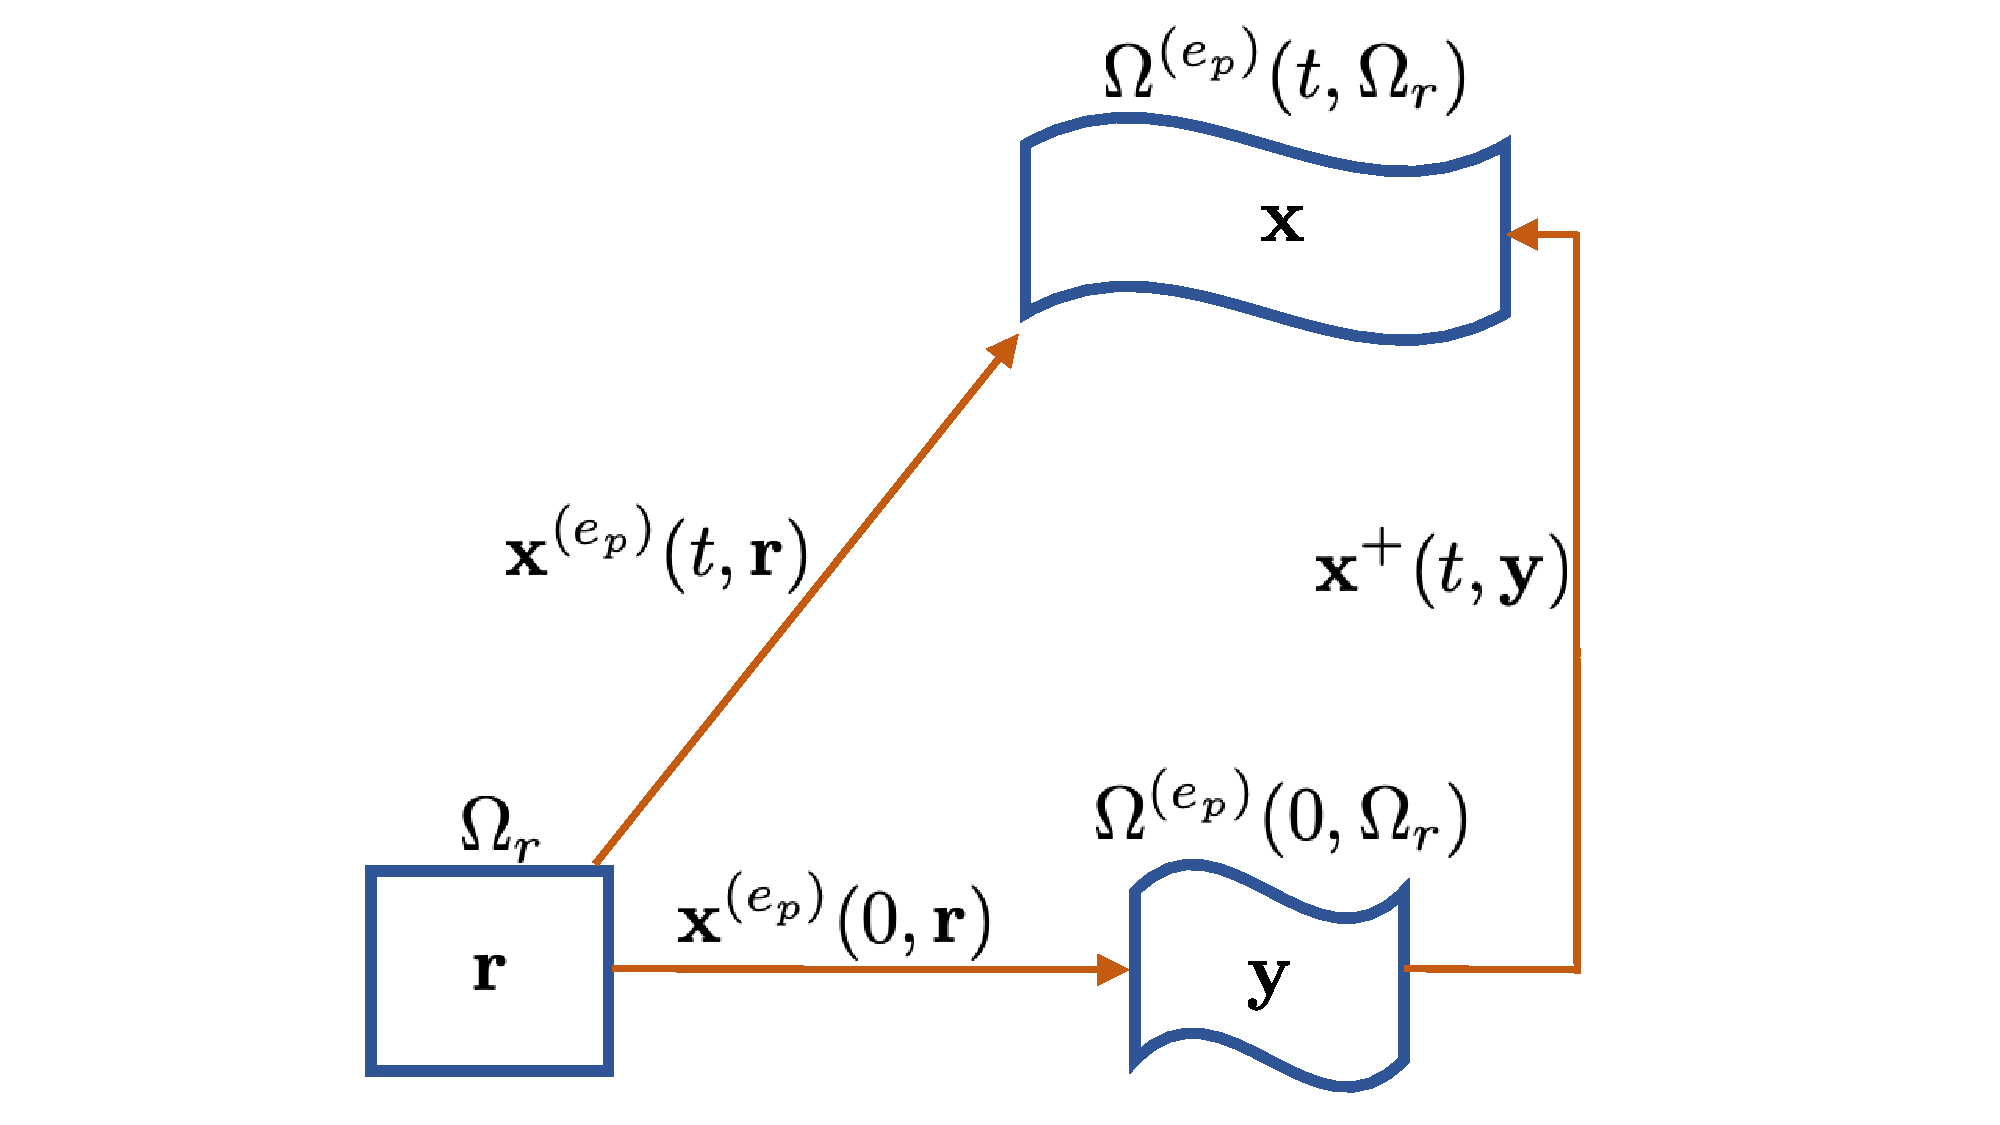
\includegraphics[width=0.7\textwidth]{../../images/three_spaces.pdf}
    \caption{Schematic of the three domains $\Omega_r$, $\Omega^{(e_p)}(t,\Omega_r)$, $\Omega^{(e_p)}(0,\Omega_r)$.}
    \label{fig:three_spaces}
 \end{figure}
We introduce the reference element as the unit square in 2D or the unit cube in 3D. The domain of this reference element is labelled as $\Omega_r$ and it doesn't change with time. We introduce the function $\Phivec^{(e_p)} = \Phivec^{(e_p)}(t,\rvec)$, which maps from points $\rvec$ in $\Omega_r$ to points in the finite element $e_p$ of the physical space. The evolving domain of the finite element $e_p$ is giving  by the function $\Omega^{(e_p)} = \Omega^{(e_p)}(t,\Omega_r)$. A depiction of these domains and their mappings is shown in \cref{fig:three_spaces}. Whereas for $\Omega^+$ we had $\Omega^+(0,\Omega_0)=\Omega_0$, for $\Omega^{(e_p)}$ the analogue does not hold, that is, $\Omega^{(e_p)}(0,\Omega_r) \ne \Omega_r$.


The mapping functions $\Phivec^{(e_p)}$ and $\xvec^+$ are related to each other as follows
\begin{equation}
    \label{eq:ref_elem_r_map}
    \Phivec^{(e_p)}(t,\rvec) = \xvec^+(t, \Phivec^{(e_p)}(0,\rvec)).
\end{equation}
The Jacobian $\Jvec^{(e_p)} = \Jvec^{(e_p)}(t,\rvec)$ is defined as 
\begin{equation}
    \Jvec^{(e_p)} = \frac{ \partial \Phivec^{(e_p)} }{ \partial \rvec },
\end{equation}
with its determinant labeled as $J^{(e_p)} = J^{(e_p)}(t,\rvec)$. Using \cref{eq:ref_elem_r_map} in the definition of $\Jvec^{(e_p)}$ we get
\begin{align*}
    \Jvec^{(e_p)} &= \left ( \frac{\partial \xvec^+}{\partial \yvec} \right )_{\yvec = \Phivec^{(e_p)}(0,\rvec)} \frac{\partial \Phivec^{(e_p)}(0,\rvec)}{\partial \rvec} \nonumber \\
    &= \left ( \Jvec^+ \right )_{\yvec = \Phivec^{(e_p)}(0,\rvec)} \Jvec^{(e_p)}_0,
\end{align*}
where $\Jvec^{(e_p)}_0 = \Jvec^{(e_p)}(0,\rvec)$.
Taking the determinant of the above gives
\begin{equation}
    \label{eq:ref_elem_det_J}
    J^{(e_p)} = \left ( J^+ \right )_{\yvec = \Phivec^{(e_p)}(0,\rvec)} J^{(e_p)}_0,
\end{equation}
where $J^{(e_p)}_0 = J^{(e_p)}(0,\rvec)$.

As a reminder, a Lagrangian variable $f^+=f^+(t,\yvec)$ is related to $f=f(t,\xvec)$ according to 
\begin{equation*}
    f^+(t,\yvec) = f(t,\xvec^+(t,\yvec)).
\end{equation*}
In an analogous manner, $f^{(e_p)}=f^{(e_p)}(t,\rvec)$ is related to $f=f(t,\xvec)$ according to
\begin{equation}
    \label{eq:ref_elem_to_eul}
    f^{(e_p)}(t,\rvec) = f(t,\Phivec^{(e_p)}(t,\rvec)).
\end{equation}
Examples of these reference-element functions include those for density $\rho^{(e_p)} = \rho^{(e_p)}(t,\rvec)$, velocity $\uvec^{(e_p)} = \uvec^{(e_p)}(t,\rvec)$, and internal energy $e^{(e_p)} = e^{(e_p)}(t,\rvec)$. Using integration by substitution and then \cref{eq:ref_elem_to_eul} we show 
\begin{align*}
    \int_{\Omega^{(e_p)}} f dV_x &= \int_{\Omega_r} f(t, \Phivec^{(e_p)}(t,\rvec)) J^{(e_p)} \, dV_r \nonumber \\
    &= \int_{\Omega_r} f^{(e_p)} J^{(e_p)} \, dV_r.
\end{align*}
In other words, integrals over elements at any time can be computed as integrals over the reference space. 

If the integrand contains a derivative, a bit of extra care is required. To show this, we'll use index notation for the sake of clarity. Consider as an example a term of the form
\begin{equation*}
    \left ( \sigmavec \cdot \nabla f \right )_{\xvec=\Phivec^{(e_p)}}= \left ( \sigma_{ij} \frac{\partial f}{\partial x_j} \right )_{\xvec = \Phivec^{(e_p)}}= \sigma_{ij}^{(e_p)} \left ( \frac{\partial f}{\partial x_j} \right )_{\xvec = \Phivec^{(e_p)}}.
\end{equation*}
We first note that
\begin{equation*}
    \frac{\partial f^{(e_p)}}{\partial r_k} = \left ( \frac{\partial f}{\partial x_i} \right )_{\xvec = \Phivec^{(e_p)}} \frac{\partial x^{(e_p)}_i}{\partial r_k} = \left ( \frac{\partial f}{\partial x_i} \right )_{\xvec = \Phivec^{(e_p)}} J^{(e_p)}_{ik}.
\end{equation*}
Upon multiplying both sides by the inverse of $\Jvec^{(e_p)}$, we get
\begin{equation*}
    \left ( \frac{\partial f}{\partial x_j} \right )_{\xvec = \Phivec^{(e_p)}} = \frac{\partial f^{(e_p)}}{\partial r_k} \left( J^{(e_p)} \right)^{-1}_{kj}.
\end{equation*}
Thus, we now have
\begin{equation*}
    \left ( \sigmavec \cdot \nabla f \right )_{\xvec=\Phivec^{(e_p)}} = \sigma^{(e_p)}_{ij}\frac{\partial f^{(e_p)}}{\partial r_k} \left( J^{(e_p)} \right)^{-1}_{kj} = \sigma^{(e_p)}_{ij} \left[ \left( J^{(e_p)} \right)^{-1} \right]^T_{jk} \frac{\partial f^{(e_p)}}{\partial r_k}.
\end{equation*}
In vector/tensor notation, the above is written as
\begin{equation*}
    \left ( \sigmavec \cdot \nabla f \right )_{\xvec=\Phivec^{(e_p)}} = \sigmavec^{(e_p)} \cdot \left[ \left( \Jvec^{(e_p)} \right)^{-1} \right]^T \cdot \nabla_\rvec f^{(e_p)}.
\end{equation*}
Thus, for the force matrix $\fvec_{ij}$ we can now write
\begin{align*}
    \int_{\Omega^{(e_p)}} \sigmavec \cdot \nabla w_i \phi_j \, dV_x &= \int_{\Omega_\rvec} \left ( \sigmavec \cdot \nabla w_i \phi_j \right )_{\xvec=\Phivec^{(e_p)}} J^{(e_p)} \, dV_r \nonumber \\
    &= \int_{\Omega_\rvec} \sigmavec^{(e_p)} \cdot \left[ \left( \Jvec^{(e_p)} \right)^{-1} \right]^T  \cdot \nabla_\rvec w^{(e_p)}_i \phi^{(e_p)}_j J^{(e_p)} \, dV_r.
\end{align*}

We also note that we can evaluate \cref{eq:evol_rho_semi_discrete} at $\yvec = \Phivec^{(e_p)}(0,\rvec)$ to obtain
\begin{equation}
    \rho^{(e_p)} = \frac{\rho^{(e_p)}_0 J^{(e_p)}_0}{J^{(e_p)}}.
\end{equation}

As with the other variables, we can define a reference basis function $w^{(e_p)}$ so that it satisfies
\begin{equation}
    w_j^{(e_p)}(t,\rvec) = w_j^+(t,\Phivec^{(e_p)}(0,\rvec)).
\end{equation}
Now, as mentioned earlier, the Lagrangian basis functions are independent of time, and as a result the reference basis functions are so as well. That is, $w^{(e_p)} = w^{(e_p)}(\rvec)$. Consider the expansion in \cref{eq:fe_exp_x}. Plugging in $\Phivec^{(e_p)}(0,\rvec)$ for $\yvec$ gives
\begin{equation}
    \label{eq:re_exp_x}
    \Phivec^{(e_p)} = \sum_j^{N_w} \hat{\xvec}_j w^{(e_p)}_j.
\end{equation}
Thus, both the Lagrangian and reference variables share the same finite-element coefficients.

%------------------------------------------------------------------------
\section{Temporal integration}
%------------------------------------------------------------------------
We now integrate forward in time the semi-discrete \cref{eq:evol_x_semi_discrete,eq:evol_vel_semi_discrete,eq:evol_energy_semi_discrete}, which we repeat below for convenience
\begin{equation}
    \tag{\ref{eq:evol_vel_semi_discrete}}
    \Mvec_\mathcal{V} \frac{d\Uvec}{dt} = -\Fvec \hat{\mathbf{1}}.
\end{equation}
\begin{equation}
    \tag{\ref{eq:evol_energy_semi_discrete}}
    \Mvec_\mathcal{E} \frac{d\Evec}{dt} = \Fvec^T \cdot \Uvec.
\end{equation}
\begin{equation}
    \tag{\ref{eq:evol_x_semi_discrete}}
    \frac{d\Xvec}{dt} = \Uvec.
\end{equation}
The equations are integrated using the RK2-average scheme of \cite{dobrev2012}, which consists of the following for the first stage
\begin{align}
    \Uvec^{n+1/2} &= \Uvec^n - \frac{\Delta t}{2} \left( \Mvec_\mathcal{V} \right)^{-1} \Fvec^n \hat{\mathbf{1}}, \nonumber \\
    \Evec^{n+1/2} &= \Evec^n + \frac{\Delta t}{2} \left( \Mvec_\mathcal{E} \right)^{-1} \left( \Fvec^n \right)^T \cdot \Uvec^{n+1/2}, \nonumber \\
    \Xvec^{n+1/2} &= \Xvec^n + \frac{\Delta t}{2} \Uvec^{n+1/2},
\end{align}
and the following for the second stage
\begin{align}
    \Uvec^{n+1} &= \Uvec^n - \Delta t \left( \Mvec_\mathcal{V} \right)^{-1} \Fvec^{n+1/2} \hat{\mathbf{1}}, \nonumber \\
    \Evec^{n+1} &= \Evec^n + \Delta t \left( \Mvec_\mathcal{E} \right)^{-1} \left( \Fvec^{n+1/2} \right)^T \cdot \bar{\Uvec}^{n+1/2}, \nonumber \\
    \Xvec^{n+1} &= \Xvec^n + \Delta t \bar{\Uvec}^{n+1/2}.
\end{align}
In the above, $\bar{\Uvec}^{n+1/2} = \left( \Uvec^n + \Uvec^{n+1} \right)/2$. In particular, this scheme is used since it conserves total energy, that is, $(IE + KE)^{n+1} - (IE + KE)^n = 0$. To prove this we first show that for the internal energy we have
\begin{align}
    \label{eq:temp_ie_change}
    IE^{n+1} - IE^n &= \hat{\mathbf{1}}^T \Mvec_\mathcal{E} \left( \Evec^{n+1} - \Evec^n \right) \nonumber \\
    &= \Delta t \hat{\mathbf{1}}^T \left( \Fvec^{n+1/2} \right)^T \cdot \bar{\Uvec}^{n+1/2}
\end{align}
For the kinetic energy we have
\begin{align}
    \label{eq:temp_ke_change}
    KE^{n+1} - KE^n &= \frac{1}{2} \left[ \left( \Uvec^{n+1} \right)^T \cdot \Mvec_\mathcal{V} \Uvec^{n+1} - \left( \Uvec^n \right)^T \cdot \Mvec_\mathcal{V} \Uvec^n \right] \nonumber \\
    &= \frac{1}{2} \left[ \left( \Uvec^{n+1} \right)^T \Mvec_\mathcal{V} \cdot \Uvec^{n+1} - \left( \Uvec^n \right)^T \Mvec_\mathcal{V} \cdot \Uvec^n \right] \nonumber \\
    &= \frac{1}{2} \left( \Uvec^{n+1} - \Uvec^n \right)^T \Mvec_\mathcal{V} \cdot \left( \Uvec^{n+1} + \Uvec^n \right) \nonumber \\ 
    &= \left( \Uvec^{n+1} - \Uvec^n \right)^T \Mvec_\mathcal{V} \cdot \bar{\Uvec}^{n+1/2} \nonumber \\
    &= \left[ - \Delta t \left( \Mvec_\mathcal{V} \right)^{-1} \Fvec^{n+1/2} \hat{\mathbf{1}} \right]^T \Mvec_\mathcal{V} \cdot \bar{\Uvec}^{n+1/2} \nonumber \\
    &= -\Delta t \hat{\mathbf{1}}^T \left( \Fvec^{n+1/2} \right)^T \left[ \left( \Mvec_\mathcal{V} \right)^{-1} \right]^T \Mvec_\mathcal{V} \cdot \bar{\Uvec}^{n+1/2} \nonumber \\
    &= -\Delta t \hat{\mathbf{1}}^T \left( \Fvec^{n+1/2} \right)^T \left[ \left( \Mvec_\mathcal{V} \right)^T \right]^{-1} \Mvec_\mathcal{V} \cdot \bar{\Uvec}^{n+1/2} \nonumber \\
    &= -\Delta t \hat{\mathbf{1}}^T \left( \Fvec^{n+1/2} \right)^T \left( \Mvec_\mathcal{V} \right)^{-1} \Mvec_\mathcal{V} \cdot \bar{\Uvec}^{n+1/2} \nonumber \\
    &= -\Delta t \hat{\mathbf{1}}^T \left( \Fvec^{n+1/2} \right)^T \cdot \bar{\Uvec}^{n+1/2}.
\end{align}
Thus, adding \cref{eq:temp_ie_change} and \cref{eq:temp_ke_change} leads to total energy conservation.

%########################################################################
\chapter{The Re-mesh Step}
%########################################################################
\begin{figure}[ht]
    \centering
    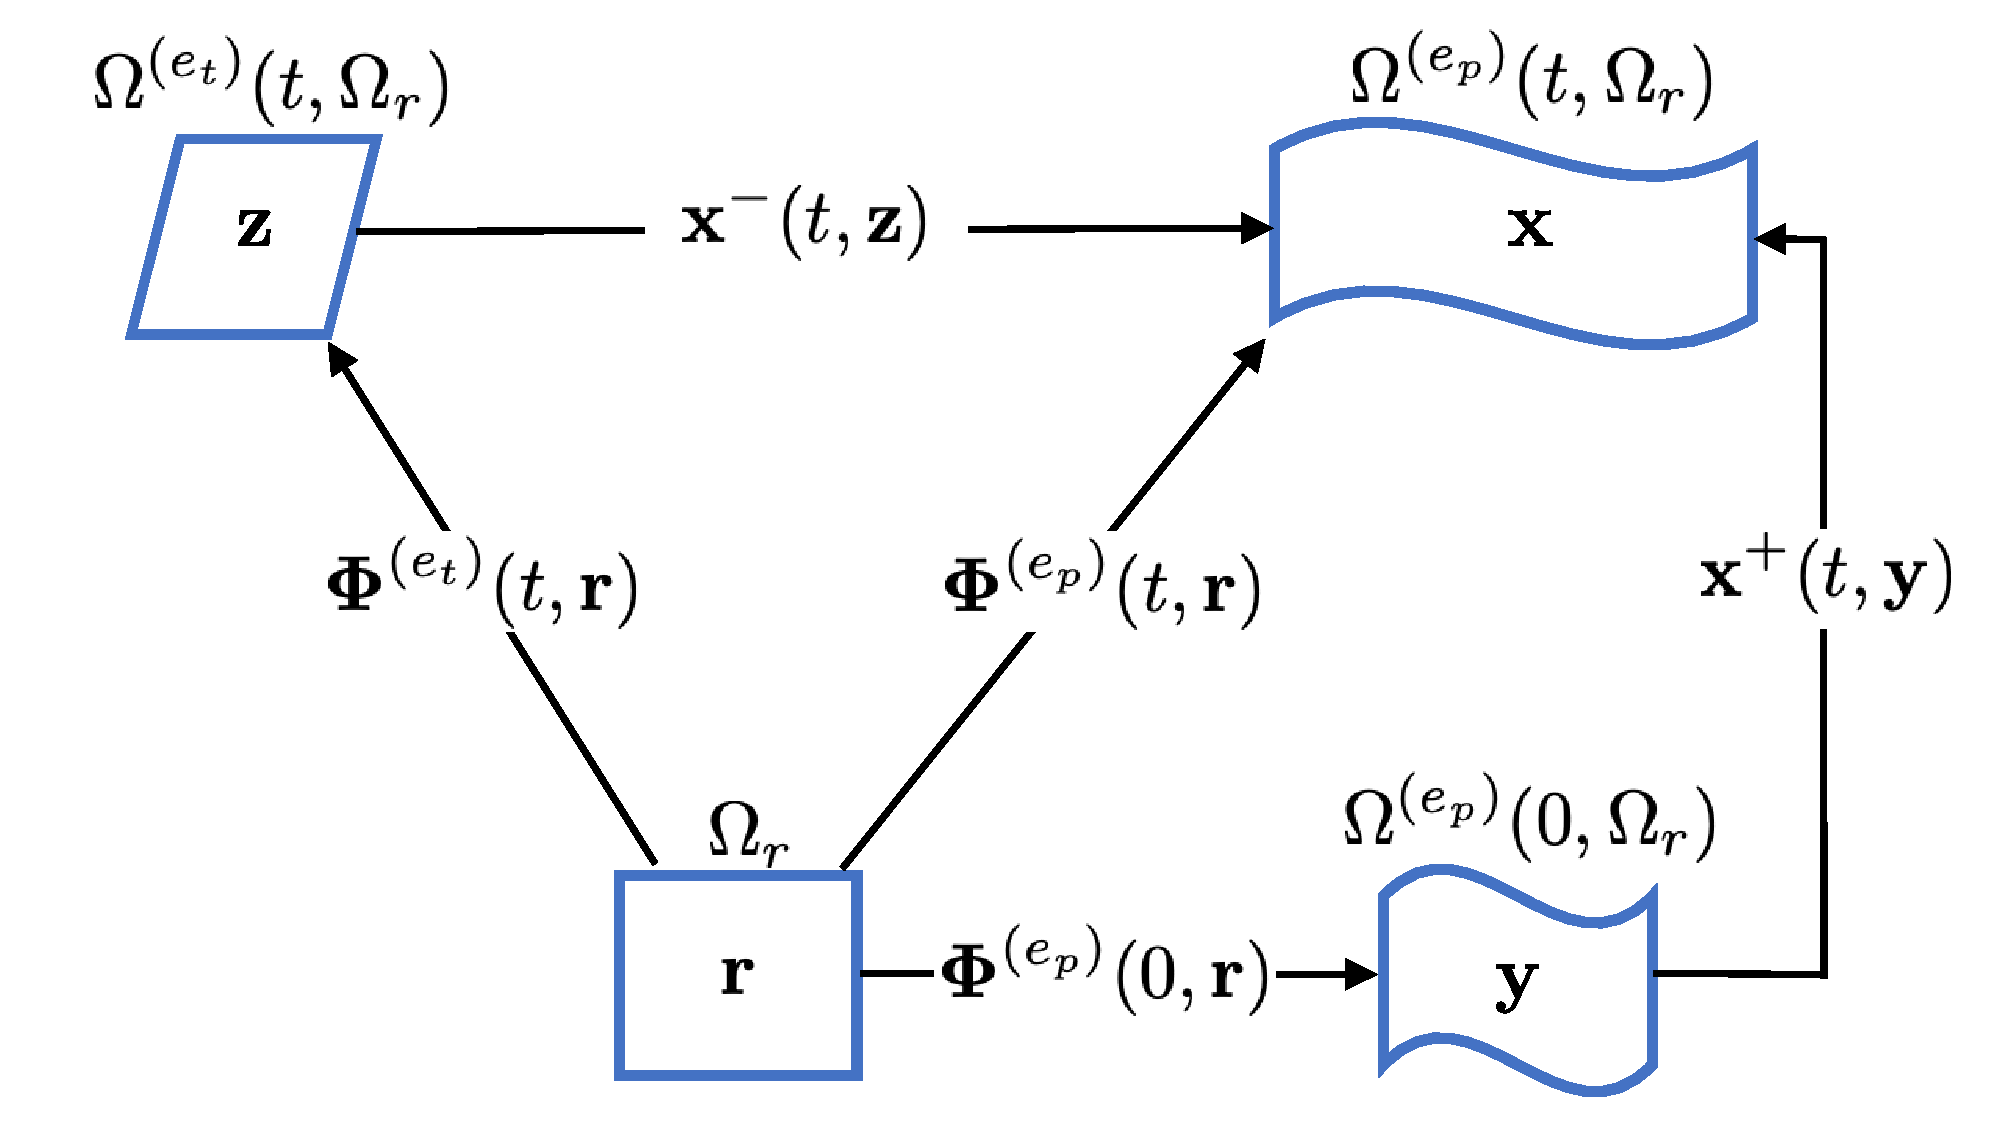
\includegraphics[width=0.7\textwidth]{../../images/four_spaces.pdf}
    \caption{Schematic of the four domains $\Omega_r$, $\Omega^{(e_p)}(t,\Omega_r)$, $\Omega^{(e_p)}(0,\Omega_r)$, $\Omega^{(e_t)}(t,\Omega_r)$.}
    \label{fig:four_spaces}
 \end{figure}
We introduce a new space, the target space, which is divided into target elements, where each corresponds to a physical element $e_p$. Consider a mapping $\Phivec^{(e_t)}=\Phivec^{(e_t)}(t,\rvec)$ from a point $\rvec$ in the reference element to a point in the target element. Also consider the mapping $\xvec^- = \xvec^-(t,\zvec)$ from a point $\zvec$ in the target space to a point in the physical space. Note that $\Phivec^{(e_p)}$, $\Phivec^{(e_t)}$, and $\xvec^-$ are related to each other according to
\begin{equation}
    \label{eq:ref_elem_z_map}
    \Phivec^{(e_p)}(t,\rvec) = \xvec^-(t,\Phivec^{(e_t)}(t,\rvec)).
\end{equation}

We define the Jacobeans as follows
\begin{equation}
    \Jvec^{(e_t)} = \frac{\partial \Phivec^{(e_t)}}{\partial \rvec},
\end{equation}
\begin{equation}
    \Jvec^- = \frac{\partial \xvec^-}{\partial \zvec}.
\end{equation}
where $\Jvec^{(e_t)} = \Jvec^{(e_t)}(t,\rvec)$ and $\Jvec^-=\Jvec^-(t,\zvec)$. Taking the derivative of \cref{eq:ref_elem_z_map} we get
\begin{equation*}
    \frac{\partial \Phivec^{(e_p)}}{\partial \rvec} = \left( \frac{ \partial \xvec^-}{\partial \zvec} \right)_{\zvec=\Phivec^{(e_t)}} \frac{ \partial \Phivec^{(e_t)} }{ \partial \rvec},
\end{equation*}
which we write as
\begin{equation*}
    \Jvec^{(e_p)} = \left( \Jvec^- \right)_{\zvec=\Phivec^{(e_t)}} \Jvec^{(e_t)}.
\end{equation*}
Multiplying both sides by the inverse of $\Jvec^{(e_t)}$ we finally get
\begin{equation}
    \left( \Jvec^- \right)_{\zvec=\Phivec^{(e_t)}} = \Jvec^{(e_p)} \left( \Jvec^{(e_t)} \right)^{-1}.
\end{equation}

Combining \cref{eq:ref_elem_r_map} and \cref{eq:ref_elem_z_map} we get
\begin{equation}
    \xvec^-(t,\Phivec^{(e_t)}(t,\rvec)) = \xvec^+(t, \Phivec^{(e_p)}(0,\rvec)).
\end{equation}
We also define a target basis function $w^{(e_t)} = w^{(e_t)}(t,\zvec)$ so that it satisfies
\begin{equation}
    w^-(t,\Phivec^{(e_t)}(t,\rvec)) = w^+(t, \Phivec^{(e_p)}(0,\rvec)).
\end{equation}
Consider the expansion in \cref{eq:fe_exp_x}. Plugging in $\Phivec^{(e_p)}(0,\rvec)$ for $\yvec$ gives
\begin{equation*}
    \xvec^-(t,\Phivec^{(e_t)}(t,\rvec)) = \sum_j^{N_w} \hat{\xvec} w^-(t,\Phivec^{(e_t)}(t,\rvec)).
\end{equation*}
Assuming this holds for any $\Phivec^{(e_t)}$ we get
\begin{equation}
    \xvec^- = \sum_j^{N_w} \hat{\xvec} w^-.
\end{equation}
Thus, both the Lagrangian and the target variables share the same finite-element coefficients.

To obtain the relaxed mesh, one minimizes the following function
\begin{equation}
    F(\Xvec) = \sum_{e_t \in \mathcal{M}_t} \int_{\Omega^{(e_t)}} \mu( \Jvec^- ) \, dV_z
\end{equation}

%########################################################################
\chapter{The Re-map Step}
%########################################################################

\bibliographystyle{plainnat}
\bibliography{library}
\end{document}